\section{Model  Class Reference}
\label{classModel}\index{Model@{Model}}
The incremental simulator model. 


{\tt \#include $<$model.h$>$}

Inheritance diagram for Model::\begin{figure}[H]
\begin{center}
\leavevmode
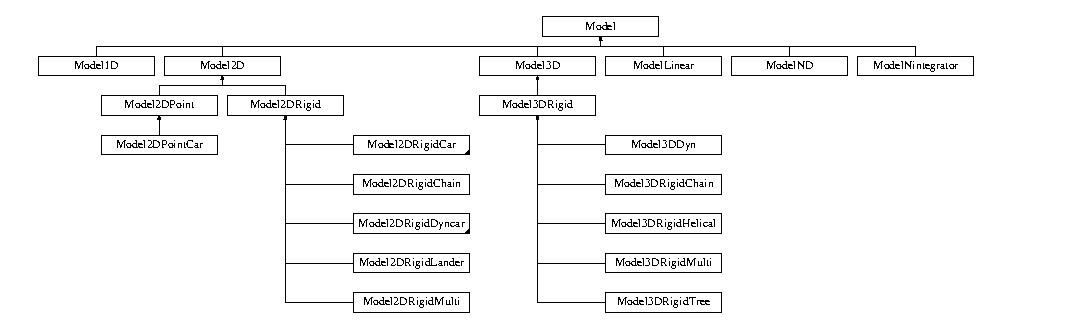
\includegraphics[height=3.97163cm]{classModel}
\end{center}
\end{figure}
\subsection*{Public Methods}
\begin{CompactItemize}
\item 
{\bf Model} (string path)
\begin{CompactList}\small\item\em Empty constructor.\item\end{CompactList}\item 
virtual {\bf $\sim$Model} ()
\begin{CompactList}\small\item\em Empty destructor.\item\end{CompactList}\item 
virtual {\bf list}$<${\bf MSLVector}$>$ {\bf Get\-Inputs} (const {\bf MSLVector} \&x)
\begin{CompactList}\small\item\em Return a {\bf list} {\rm (p.\,\pageref{classlist})} of inputs, which may depend on state.\item\end{CompactList}\item 
virtual {\bf MSLVector} {\bf State\-Transition\-Equation} (const {\bf MSLVector} \&x, const {\bf MSLVector} \&u)=0
\begin{CompactList}\small\item\em The state transition equation, or equations of motion, xdot=f(x,u).\item\end{CompactList}\item 
virtual bool {\bf Satisfied} (const {\bf MSLVector} \&x)
\begin{CompactList}\small\item\em Test whether global state-space constraints are satisfied.\item\end{CompactList}\item 
virtual {\bf MSLVector} {\bf Integrate} (const {\bf MSLVector} \&x, const {\bf MSLVector} \&u, const double \&h)=0
\begin{CompactList}\small\item\em Perform integration from state x, using input u, over time step h.\item\end{CompactList}\item 
virtual {\bf MSLVector} {\bf Linear\-Interpolate} (const {\bf MSLVector} \&x1, const {\bf MSLVector} \&x2, const double \&a)
\begin{CompactList}\small\item\em Linearly interpolate two state while respecting topology.\item\end{CompactList}\item 
virtual {\bf MSLVector} {\bf State\-Difference} (const {\bf MSLVector} \&x1, const {\bf MSLVector} \&x2)
\begin{CompactList}\small\item\em Compute a {\bf MSLVector} {\rm (p.\,\pageref{classMSLVector})} based on x2-x1. In R$^\wedge$n, the states are simply subtracted to make the {\bf MSLVector} {\rm (p.\,\pageref{classMSLVector})}. This method exists to make things work correctly for other state-space topologies.\item\end{CompactList}\item 
virtual {\bf MSLVector} {\bf State\-To\-Configuration} (const {\bf MSLVector} \&x)
\begin{CompactList}\small\item\em A method that converts a Model state in to a {\bf Geom} {\rm (p.\,\pageref{classGeom})} configuration.\item\end{CompactList}\item 
virtual double {\bf Metric} (const {\bf MSLVector} \&x1, const {\bf MSLVector} \&x2)
\begin{CompactList}\small\item\em A distance metric, which is Euclidean in the base class.\item\end{CompactList}\item 
virtual void {\bf Partialf\_\-x} (const {\bf MSLVector} \&x, const {\bf MSLVector} \&u, {\bf MSLMatrix} \&m)
\begin{CompactList}\small\item\em Partial with respect to x of the state transition equation.\item\end{CompactList}\item 
virtual void {\bf Partialf\_\-u} (const {\bf MSLVector} \&x, const {\bf MSLVector} \&u, {\bf MSLMatrix} \&m)
\begin{CompactList}\small\item\em Partial with respect to u of the state transition equation.\item\end{CompactList}\item 
virtual void {\bf L} (const {\bf MSLVector} \&x, const {\bf MSLVector} \&u, double \&l)
\begin{CompactList}\small\item\em A cost or loss function, to be used in optimization problems.\item\end{CompactList}\item 
virtual void {\bf Partial\-L\_\-x} (const {\bf MSLVector} \&x, const {\bf MSLVector} \&u, {\bf MSLMatrix} \&m)
\begin{CompactList}\small\item\em Partial of the loss with respect to x.\item\end{CompactList}\item 
virtual void {\bf Partial\-L\_\-u} (const {\bf MSLVector} \&x, const {\bf MSLVector} \&u, {\bf MSLMatrix} \&m)
\begin{CompactList}\small\item\em Partial of the loss with respect to u.\item\end{CompactList}\item 
virtual void {\bf Phi} (const {\bf MSLVector} \&x, const {\bf MSLVector} \&u, const {\bf MSLVector} \&goalstate, double \&phi)
\begin{CompactList}\small\item\em The final-state cost or loss.\item\end{CompactList}\item 
virtual void {\bf Partial\-Phi\_\-x} (const {\bf MSLVector} \&x, const {\bf MSLVector} \&u, const {\bf MSLVector} \&goalstate, {\bf MSLMatrix} \&m)
\begin{CompactList}\small\item\em Partial of the final-state loss with respect to x.\item\end{CompactList}\item 
virtual void {\bf Partial\-Phi\_\-t} (const {\bf MSLVector} \&x, const {\bf MSLVector} \&u, const {\bf MSLVector} \&goalstate, {\bf MSLMatrix} \&m)
\begin{CompactList}\small\item\em Partial of the final-state loss with respect to u.\item\end{CompactList}\item 
virtual void {\bf Psi} (const {\bf MSLVector} \&x, const {\bf MSLVector} \&goalstate, {\bf MSLVector} \&psi)
\begin{CompactList}\small\item\em An error {\bf MSLVector} {\rm (p.\,\pageref{classMSLVector})} that compares a goal state to a given state.\item\end{CompactList}\item 
virtual void {\bf Partial\-Psi\_\-x} (const {\bf MSLVector} \&x, const {\bf MSLVector} \&u, {\bf MSLMatrix} \&m)
\begin{CompactList}\small\item\em Partial of the error {\bf MSLVector} {\rm (p.\,\pageref{classMSLVector})} with respect to x.\item\end{CompactList}\item 
virtual void {\bf Partial\-Psi\_\-t} (const {\bf MSLVector} \&x, const {\bf MSLVector} \&u, {\bf MSLMatrix} \&m)
\begin{CompactList}\small\item\em Partial of the error {\bf MSLVector} {\rm (p.\,\pageref{classMSLVector})} with respect to time.\item\end{CompactList}\end{CompactItemize}
\subsection*{Public Attributes}
\begin{CompactItemize}
\item 
string {\bf File\-Path}
\begin{CompactList}\small\item\em This file path is used for all file reads.\item\end{CompactList}\item 
{\bf MSLVector} {\bf Lower\-State}
\begin{CompactList}\small\item\em {\bf MSLVector} {\rm (p.\,\pageref{classMSLVector})} of minimum values for each state variable.\item\end{CompactList}\item 
{\bf MSLVector} {\bf Upper\-State}
\begin{CompactList}\small\item\em {\bf MSLVector} {\rm (p.\,\pageref{classMSLVector})} of maximum values for each state variable.\item\end{CompactList}\item 
{\bf MSLVector} {\bf Lower\-Input}
\begin{CompactList}\small\item\em {\bf MSLVector} {\rm (p.\,\pageref{classMSLVector})} of minimum values for each input variable.\item\end{CompactList}\item 
{\bf MSLVector} {\bf Upper\-Input}
\begin{CompactList}\small\item\em {\bf MSLVector} {\rm (p.\,\pageref{classMSLVector})} of maximum values for each input variable.\item\end{CompactList}\item 
int {\bf State\-Dim}
\begin{CompactList}\small\item\em The dimension of the state space.\item\end{CompactList}\item 
int {\bf Input\-Dim}
\begin{CompactList}\small\item\em The dimension of the input space.\item\end{CompactList}\end{CompactItemize}
\subsection*{Protected Methods}
\begin{CompactItemize}
\item 
{\bf MSLVector} {\bf Runge\-Kutta\-Integrate} (const {\bf MSLVector} \&x, const {\bf MSLVector} \&u, const double \&h)
\begin{CompactList}\small\item\em Integrate xdot using 4th-order Runge-Kutta.\item\end{CompactList}\item 
{\bf MSLVector} {\bf Euler\-Integrate} (const {\bf MSLVector} \&x, const {\bf MSLVector} \&u, const double \&h)
\begin{CompactList}\small\item\em Integrate xdot using Euler integration.\item\end{CompactList}\end{CompactItemize}
\subsection*{Protected Attributes}
\begin{CompactItemize}
\item 
double {\bf Model\-Delta\-T}
\begin{CompactList}\small\item\em The time interval to use for numerical integration (affects accuracy).\item\end{CompactList}\item 
{\bf list}$<${\bf MSLVector}$>$ {\bf Inputs}
\begin{CompactList}\small\item\em The complete set of inputs.\item\end{CompactList}\end{CompactItemize}


\subsection{Detailed Description}
The incremental simulator model.

The Model classes contain incremental simulators that model the kinematics and dynamics of a variety of mechanical systems. The methods allow planning algorithms to compute the future system state, given the current state, an interval of time, and a control input applied over that interval. (The planning algorithms select the appropriate inputs using this information.) Using object-oriented class derivations, a wide variety of simulators can be included. 



\subsection{Constructor \& Destructor Documentation}
\index{Model@{Model}!Model@{Model}}
\index{Model@{Model}!Model@{Model}}
\subsubsection{\setlength{\rightskip}{0pt plus 5cm}Model::Model (string {\em path})}\label{classModel_a0}


Empty constructor.

\index{Model@{Model}!~Model@{$\sim$Model}}
\index{~Model@{$\sim$Model}!Model@{Model}}
\subsubsection{\setlength{\rightskip}{0pt plus 5cm}Model::$\sim$Model ()\hspace{0.3cm}{\tt  [inline, virtual]}}\label{classModel_a1}


Empty destructor.



\subsection{Member Function Documentation}
\index{Model@{Model}!EulerIntegrate@{EulerIntegrate}}
\index{EulerIntegrate@{EulerIntegrate}!Model@{Model}}
\subsubsection{\setlength{\rightskip}{0pt plus 5cm}{\bf MSLVector} Model::Euler\-Integrate (const {\bf MSLVector} \& {\em x}, const {\bf MSLVector} \& {\em u}, const double \& {\em h})\hspace{0.3cm}{\tt  [protected]}}\label{classModel_b1}


Integrate xdot using Euler integration.

\index{Model@{Model}!GetInputs@{GetInputs}}
\index{GetInputs@{GetInputs}!Model@{Model}}
\subsubsection{\setlength{\rightskip}{0pt plus 5cm}{\bf list}$<$ {\bf MSLVector} $>$ Model::Get\-Inputs (const {\bf MSLVector} \& {\em x})\hspace{0.3cm}{\tt  [virtual]}}\label{classModel_a2}


Return a {\bf list} {\rm (p.\,\pageref{classlist})} of inputs, which may depend on state.

\index{Model@{Model}!Integrate@{Integrate}}
\index{Integrate@{Integrate}!Model@{Model}}
\subsubsection{\setlength{\rightskip}{0pt plus 5cm}{\bf MSLVector} Model::Integrate (const {\bf MSLVector} \& {\em x}, const {\bf MSLVector} \& {\em u}, const double \& {\em h})\hspace{0.3cm}{\tt  [pure virtual]}}\label{classModel_a5}


Perform integration from state x, using input u, over time step h.



Reimplemented in {\bf Model2DPoint} {\rm (p.\,\pageref{classModel2DPoint_a2})}, {\bf Model2DPoint\-Car} {\rm (p.\,\pageref{classModel2DPointCar_a2})}, {\bf Model2DRigid} {\rm (p.\,\pageref{classModel2DRigid_a2})}, {\bf Model2DRigid\-Car\-Smooth} {\rm (p.\,\pageref{classModel2DRigidCarSmooth_a3})}, {\bf Model2DRigid\-Dyncar} {\rm (p.\,\pageref{classModel2DRigidDyncar_a2})}, {\bf Model2DRigid\-Lander} {\rm (p.\,\pageref{classModel2DRigidLander_a2})}, {\bf Model3DRigid} {\rm (p.\,\pageref{classModel3DRigid_a2})}, {\bf Model\-Car\-Dyn\-Rollover} {\rm (p.\,\pageref{classModelCarDynRollover_a5})}, {\bf Model1D} {\rm (p.\,\pageref{classModel1D_a3})}, {\bf Model\-Linear} {\rm (p.\,\pageref{classModelLinear_a3})}, {\bf Model\-ND} {\rm (p.\,\pageref{classModelND_a3})}, {\bf Model\-Nintegrator} {\rm (p.\,\pageref{classModelNintegrator_a3})}, and {\bf Model3DRigid\-Helical} {\rm (p.\,\pageref{classModel3DRigidHelical_a3})}.\index{Model@{Model}!L@{L}}
\index{L@{L}!Model@{Model}}
\subsubsection{\setlength{\rightskip}{0pt plus 5cm}void Model::L (const {\bf MSLVector} \& {\em x}, const {\bf MSLVector} \& {\em u}, double \& {\em l})\hspace{0.3cm}{\tt  [inline, virtual]}}\label{classModel_a12}


A cost or loss function, to be used in optimization problems.

\index{Model@{Model}!LinearInterpolate@{LinearInterpolate}}
\index{LinearInterpolate@{LinearInterpolate}!Model@{Model}}
\subsubsection{\setlength{\rightskip}{0pt plus 5cm}{\bf MSLVector} Model::Linear\-Interpolate (const {\bf MSLVector} \& {\em x1}, const {\bf MSLVector} \& {\em x2}, const double \& {\em a})\hspace{0.3cm}{\tt  [virtual]}}\label{classModel_a6}


Linearly interpolate two state while respecting topology.

If a=0, then x1 is returned; if a=1, then x2 is returned. All intermediate values of \$a $\backslash$in [0,1]\$ yield intermediate states. This method is defined by Model. 

Reimplemented in {\bf Model2DRigid} {\rm (p.\,\pageref{classModel2DRigid_a4})}, {\bf Model2DRigid\-Dyncar} {\rm (p.\,\pageref{classModel2DRigidDyncar_a6})}, {\bf Model2DRigid\-Multi} {\rm (p.\,\pageref{classModel2DRigidMulti_a4})}, {\bf Model2DRigid\-Chain} {\rm (p.\,\pageref{classModel2DRigidChain_a4})}, {\bf Model3DRigid} {\rm (p.\,\pageref{classModel3DRigid_a5})}, {\bf Model3DRigid\-Multi} {\rm (p.\,\pageref{classModel3DRigidMulti_a3})}, {\bf Model3DRigid\-Chain} {\rm (p.\,\pageref{classModel3DRigidChain_a4})}, {\bf Model3DRigid\-Tree} {\rm (p.\,\pageref{classModel3DRigidTree_a4})}, and {\bf Model\-Car\-Dyn\-Smooth\-Rollover} {\rm (p.\,\pageref{classModelCarDynSmoothRollover_a5})}.\index{Model@{Model}!Metric@{Metric}}
\index{Metric@{Metric}!Model@{Model}}
\subsubsection{\setlength{\rightskip}{0pt plus 5cm}double Model::Metric (const {\bf MSLVector} \& {\em x1}, const {\bf MSLVector} \& {\em x2})\hspace{0.3cm}{\tt  [virtual]}}\label{classModel_a9}


A distance metric, which is Euclidean in the base class.



Reimplemented in {\bf Model2DPoint} {\rm (p.\,\pageref{classModel2DPoint_a4})}, {\bf Model2DPoint\-Car} {\rm (p.\,\pageref{classModel2DPointCar_a4})}, {\bf Model2DRigid} {\rm (p.\,\pageref{classModel2DRigid_a5})}, {\bf Model2DRigid\-Car\-Smooth} {\rm (p.\,\pageref{classModel2DRigidCarSmooth_a4})}, {\bf Model2DRigid\-Car\-Smooth\-Trailer} {\rm (p.\,\pageref{classModel2DRigidCarSmoothTrailer_a3})}, {\bf Model2DRigid\-Car\-Smooth2Trailers} {\rm (p.\,\pageref{classModel2DRigidCarSmooth2Trailers_a3})}, {\bf Model2DRigid\-Car\-Smooth3Trailers} {\rm (p.\,\pageref{classModel2DRigidCarSmooth3Trailers_a3})}, {\bf Model2DRigid\-Dyncar} {\rm (p.\,\pageref{classModel2DRigidDyncar_a5})}, {\bf Model2DRigid\-Lander} {\rm (p.\,\pageref{classModel2DRigidLander_a5})}, {\bf Model2DRigid\-Multi} {\rm (p.\,\pageref{classModel2DRigidMulti_a2})}, {\bf Model2DRigid\-Chain} {\rm (p.\,\pageref{classModel2DRigidChain_a5})}, {\bf Model3DRigid} {\rm (p.\,\pageref{classModel3DRigid_a4})}, {\bf Model3DRigid\-Multi} {\rm (p.\,\pageref{classModel3DRigidMulti_a2})}, {\bf Model3DRigid\-Chain} {\rm (p.\,\pageref{classModel3DRigidChain_a5})}, {\bf Model3DRigid\-Tree} {\rm (p.\,\pageref{classModel3DRigidTree_a5})}, {\bf Model\-Car\-Dyn} {\rm (p.\,\pageref{classModelCarDyn_a3})}, {\bf Model\-Car\-Dyn\-Ntire} {\rm (p.\,\pageref{classModelCarDynNtire_a3})}, {\bf Model\-Car\-Dyn\-Rollover} {\rm (p.\,\pageref{classModelCarDynRollover_a6})}, {\bf Model\-Car\-Dyn\-Smooth\-Rollover} {\rm (p.\,\pageref{classModelCarDynSmoothRollover_a4})}, and {\bf Model1D} {\rm (p.\,\pageref{classModel1D_a5})}.\index{Model@{Model}!PartialL_u@{PartialL\_\-u}}
\index{PartialL_u@{PartialL\_\-u}!Model@{Model}}
\subsubsection{\setlength{\rightskip}{0pt plus 5cm}void Model::Partial\-L\_\-u (const {\bf MSLVector} \& {\em x}, const {\bf MSLVector} \& {\em u}, {\bf MSLMatrix} \& {\em m})\hspace{0.3cm}{\tt  [inline, virtual]}}\label{classModel_a14}


Partial of the loss with respect to u.

\index{Model@{Model}!PartialL_x@{PartialL\_\-x}}
\index{PartialL_x@{PartialL\_\-x}!Model@{Model}}
\subsubsection{\setlength{\rightskip}{0pt plus 5cm}void Model::Partial\-L\_\-x (const {\bf MSLVector} \& {\em x}, const {\bf MSLVector} \& {\em u}, {\bf MSLMatrix} \& {\em m})\hspace{0.3cm}{\tt  [inline, virtual]}}\label{classModel_a13}


Partial of the loss with respect to x.

\index{Model@{Model}!PartialPhi_t@{PartialPhi\_\-t}}
\index{PartialPhi_t@{PartialPhi\_\-t}!Model@{Model}}
\subsubsection{\setlength{\rightskip}{0pt plus 5cm}void Model::Partial\-Phi\_\-t (const {\bf MSLVector} \& {\em x}, const {\bf MSLVector} \& {\em u}, const {\bf MSLVector} \& {\em goalstate}, {\bf MSLMatrix} \& {\em m})\hspace{0.3cm}{\tt  [inline, virtual]}}\label{classModel_a17}


Partial of the final-state loss with respect to u.

\index{Model@{Model}!PartialPhi_x@{PartialPhi\_\-x}}
\index{PartialPhi_x@{PartialPhi\_\-x}!Model@{Model}}
\subsubsection{\setlength{\rightskip}{0pt plus 5cm}void Model::Partial\-Phi\_\-x (const {\bf MSLVector} \& {\em x}, const {\bf MSLVector} \& {\em u}, const {\bf MSLVector} \& {\em goalstate}, {\bf MSLMatrix} \& {\em m})\hspace{0.3cm}{\tt  [inline, virtual]}}\label{classModel_a16}


Partial of the final-state loss with respect to x.

\index{Model@{Model}!PartialPsi_t@{PartialPsi\_\-t}}
\index{PartialPsi_t@{PartialPsi\_\-t}!Model@{Model}}
\subsubsection{\setlength{\rightskip}{0pt plus 5cm}void Model::Partial\-Psi\_\-t (const {\bf MSLVector} \& {\em x}, const {\bf MSLVector} \& {\em u}, {\bf MSLMatrix} \& {\em m})\hspace{0.3cm}{\tt  [inline, virtual]}}\label{classModel_a20}


Partial of the error {\bf MSLVector} {\rm (p.\,\pageref{classMSLVector})} with respect to time.

\index{Model@{Model}!PartialPsi_x@{PartialPsi\_\-x}}
\index{PartialPsi_x@{PartialPsi\_\-x}!Model@{Model}}
\subsubsection{\setlength{\rightskip}{0pt plus 5cm}void Model::Partial\-Psi\_\-x (const {\bf MSLVector} \& {\em x}, const {\bf MSLVector} \& {\em u}, {\bf MSLMatrix} \& {\em m})\hspace{0.3cm}{\tt  [inline, virtual]}}\label{classModel_a19}


Partial of the error {\bf MSLVector} {\rm (p.\,\pageref{classMSLVector})} with respect to x.

\index{Model@{Model}!Partialf_u@{Partialf\_\-u}}
\index{Partialf_u@{Partialf\_\-u}!Model@{Model}}
\subsubsection{\setlength{\rightskip}{0pt plus 5cm}void Model::Partialf\_\-u (const {\bf MSLVector} \& {\em x}, const {\bf MSLVector} \& {\em u}, {\bf MSLMatrix} \& {\em m})\hspace{0.3cm}{\tt  [inline, virtual]}}\label{classModel_a11}


Partial with respect to u of the state transition equation.

\index{Model@{Model}!Partialf_x@{Partialf\_\-x}}
\index{Partialf_x@{Partialf\_\-x}!Model@{Model}}
\subsubsection{\setlength{\rightskip}{0pt plus 5cm}void Model::Partialf\_\-x (const {\bf MSLVector} \& {\em x}, const {\bf MSLVector} \& {\em u}, {\bf MSLMatrix} \& {\em m})\hspace{0.3cm}{\tt  [inline, virtual]}}\label{classModel_a10}


Partial with respect to x of the state transition equation.

\index{Model@{Model}!Phi@{Phi}}
\index{Phi@{Phi}!Model@{Model}}
\subsubsection{\setlength{\rightskip}{0pt plus 5cm}void Model::Phi (const {\bf MSLVector} \& {\em x}, const {\bf MSLVector} \& {\em u}, const {\bf MSLVector} \& {\em goalstate}, double \& {\em phi})\hspace{0.3cm}{\tt  [inline, virtual]}}\label{classModel_a15}


The final-state cost or loss.

\index{Model@{Model}!Psi@{Psi}}
\index{Psi@{Psi}!Model@{Model}}
\subsubsection{\setlength{\rightskip}{0pt plus 5cm}void Model::Psi (const {\bf MSLVector} \& {\em x}, const {\bf MSLVector} \& {\em goalstate}, {\bf MSLVector} \& {\em psi})\hspace{0.3cm}{\tt  [inline, virtual]}}\label{classModel_a18}


An error {\bf MSLVector} {\rm (p.\,\pageref{classMSLVector})} that compares a goal state to a given state.

\index{Model@{Model}!RungeKuttaIntegrate@{RungeKuttaIntegrate}}
\index{RungeKuttaIntegrate@{RungeKuttaIntegrate}!Model@{Model}}
\subsubsection{\setlength{\rightskip}{0pt plus 5cm}{\bf MSLVector} Model::Runge\-Kutta\-Integrate (const {\bf MSLVector} \& {\em x}, const {\bf MSLVector} \& {\em u}, const double \& {\em h})\hspace{0.3cm}{\tt  [protected]}}\label{classModel_b0}


Integrate xdot using 4th-order Runge-Kutta.

\index{Model@{Model}!Satisfied@{Satisfied}}
\index{Satisfied@{Satisfied}!Model@{Model}}
\subsubsection{\setlength{\rightskip}{0pt plus 5cm}bool Model::Satisfied (const {\bf MSLVector} \& {\em x})\hspace{0.3cm}{\tt  [virtual]}}\label{classModel_a4}


Test whether global state-space constraints are satisfied.



Reimplemented in {\bf Model2DRigid\-Car\-Smooth} {\rm (p.\,\pageref{classModel2DRigidCarSmooth_a6})}, {\bf Model2DRigid\-Car\-Smooth\-Trailer} {\rm (p.\,\pageref{classModel2DRigidCarSmoothTrailer_a5})}, {\bf Model2DRigid\-Car\-Smooth2Trailers} {\rm (p.\,\pageref{classModel2DRigidCarSmooth2Trailers_a5})}, {\bf Model2DRigid\-Car\-Smooth3Trailers} {\rm (p.\,\pageref{classModel2DRigidCarSmooth3Trailers_a5})}, {\bf Model2DRigid\-Chain} {\rm (p.\,\pageref{classModel2DRigidChain_a6})}, {\bf Model3DRigid\-Chain} {\rm (p.\,\pageref{classModel3DRigidChain_a6})}, {\bf Model3DRigid\-Tree} {\rm (p.\,\pageref{classModel3DRigidTree_a6})}, {\bf Model3DDyn} {\rm (p.\,\pageref{classModel3DDyn_a3})}, {\bf Model\-Car} {\rm (p.\,\pageref{classModelCar_a3})}, and {\bf Model\-Car\-Dyn\-Rollover} {\rm (p.\,\pageref{classModelCarDynRollover_a8})}.\index{Model@{Model}!StateDifference@{StateDifference}}
\index{StateDifference@{StateDifference}!Model@{Model}}
\subsubsection{\setlength{\rightskip}{0pt plus 5cm}{\bf MSLVector} Model::State\-Difference (const {\bf MSLVector} \& {\em x1}, const {\bf MSLVector} \& {\em x2})\hspace{0.3cm}{\tt  [virtual]}}\label{classModel_a7}


Compute a {\bf MSLVector} {\rm (p.\,\pageref{classMSLVector})} based on x2-x1. In R$^\wedge$n, the states are simply subtracted to make the {\bf MSLVector} {\rm (p.\,\pageref{classMSLVector})}. This method exists to make things work correctly for other state-space topologies.

\index{Model@{Model}!StateToConfiguration@{StateToConfiguration}}
\index{StateToConfiguration@{StateToConfiguration}!Model@{Model}}
\subsubsection{\setlength{\rightskip}{0pt plus 5cm}{\bf MSLVector} Model::State\-To\-Configuration (const {\bf MSLVector} \& {\em x})\hspace{0.3cm}{\tt  [virtual]}}\label{classModel_a8}


A method that converts a Model state in to a {\bf Geom} {\rm (p.\,\pageref{classGeom})} configuration.



Reimplemented in {\bf Model2D} {\rm (p.\,\pageref{classModel2D_a2})}, {\bf Model2DRigid} {\rm (p.\,\pageref{classModel2DRigid_a6})}, {\bf Model2DRigid\-Car\-Smooth} {\rm (p.\,\pageref{classModel2DRigidCarSmooth_a5})}, {\bf Model2DRigid\-Car\-Smooth\-Trailer} {\rm (p.\,\pageref{classModel2DRigidCarSmoothTrailer_a4})}, {\bf Model2DRigid\-Car\-Smooth2Trailers} {\rm (p.\,\pageref{classModel2DRigidCarSmooth2Trailers_a4})}, {\bf Model2DRigid\-Car\-Smooth3Trailers} {\rm (p.\,\pageref{classModel2DRigidCarSmooth3Trailers_a4})}, {\bf Model2DRigid\-Dyncar} {\rm (p.\,\pageref{classModel2DRigidDyncar_a3})}, {\bf Model2DRigid\-Lander} {\rm (p.\,\pageref{classModel2DRigidLander_a3})}, {\bf Model2DRigid\-Multi} {\rm (p.\,\pageref{classModel2DRigidMulti_a3})}, {\bf Model2DRigid\-Chain} {\rm (p.\,\pageref{classModel2DRigidChain_a2})}, {\bf Model3DRigid\-Chain} {\rm (p.\,\pageref{classModel3DRigidChain_a3})}, {\bf Model3DRigid\-Tree} {\rm (p.\,\pageref{classModel3DRigidTree_a3})}, {\bf Model\-Car} {\rm (p.\,\pageref{classModelCar_a2})}, {\bf Model\-Car\-Smooth} {\rm (p.\,\pageref{classModelCarSmooth_a2})}, {\bf Model\-Car\-Dyn} {\rm (p.\,\pageref{classModelCarDyn_a2})}, {\bf Model\-Car\-Dyn\-Ntire} {\rm (p.\,\pageref{classModelCarDynNtire_a2})}, {\bf Model\-Car\-Dyn\-Rollover} {\rm (p.\,\pageref{classModelCarDynRollover_a4})}, {\bf Model\-Car\-Dyn\-Smooth\-Rollover} {\rm (p.\,\pageref{classModelCarDynSmoothRollover_a3})}, {\bf Model1D} {\rm (p.\,\pageref{classModel1D_a2})}, {\bf Model\-Linear} {\rm (p.\,\pageref{classModelLinear_a2})}, {\bf Model\-ND} {\rm (p.\,\pageref{classModelND_a2})}, and {\bf Model\-Nintegrator} {\rm (p.\,\pageref{classModelNintegrator_a2})}.\index{Model@{Model}!StateTransitionEquation@{StateTransitionEquation}}
\index{StateTransitionEquation@{StateTransitionEquation}!Model@{Model}}
\subsubsection{\setlength{\rightskip}{0pt plus 5cm}{\bf MSLVector} Model::State\-Transition\-Equation (const {\bf MSLVector} \& {\em x}, const {\bf MSLVector} \& {\em u})\hspace{0.3cm}{\tt  [pure virtual]}}\label{classModel_a3}


The state transition equation, or equations of motion, xdot=f(x,u).



Reimplemented in {\bf Model2DPoint} {\rm (p.\,\pageref{classModel2DPoint_a3})}, {\bf Model2DPoint\-Car} {\rm (p.\,\pageref{classModel2DPointCar_a3})}, {\bf Model2DRigid} {\rm (p.\,\pageref{classModel2DRigid_a3})}, {\bf Model2DRigid\-Car} {\rm (p.\,\pageref{classModel2DRigidCar_a2})}, {\bf Model2DRigid\-Car\-Smooth} {\rm (p.\,\pageref{classModel2DRigidCarSmooth_a2})}, {\bf Model2DRigid\-Car\-Smooth\-Trailer} {\rm (p.\,\pageref{classModel2DRigidCarSmoothTrailer_a2})}, {\bf Model2DRigid\-Car\-Smooth2Trailers} {\rm (p.\,\pageref{classModel2DRigidCarSmooth2Trailers_a2})}, {\bf Model2DRigid\-Car\-Smooth3Trailers} {\rm (p.\,\pageref{classModel2DRigidCarSmooth3Trailers_a2})}, {\bf Model2DRigid\-Dyncar} {\rm (p.\,\pageref{classModel2DRigidDyncar_a4})}, {\bf Model2DRigid\-Dyncar\-Ntire} {\rm (p.\,\pageref{classModel2DRigidDyncarNtire_a2})}, {\bf Model2DRigid\-Lander} {\rm (p.\,\pageref{classModel2DRigidLander_a4})}, {\bf Model2DRigid\-Chain} {\rm (p.\,\pageref{classModel2DRigidChain_a3})}, {\bf Model3DRigid} {\rm (p.\,\pageref{classModel3DRigid_a3})}, {\bf Model3DRigid\-Chain} {\rm (p.\,\pageref{classModel3DRigidChain_a2})}, {\bf Model3DRigid\-Tree} {\rm (p.\,\pageref{classModel3DRigidTree_a2})}, {\bf Model3DDyn} {\rm (p.\,\pageref{classModel3DDyn_a2})}, {\bf Model\-Car\-Dyn\-Rollover} {\rm (p.\,\pageref{classModelCarDynRollover_a3})}, {\bf Model\-Car\-Dyn\-Smooth\-Rollover} {\rm (p.\,\pageref{classModelCarDynSmoothRollover_a2})}, {\bf Model1D} {\rm (p.\,\pageref{classModel1D_a4})}, {\bf Model\-Linear} {\rm (p.\,\pageref{classModelLinear_a4})}, {\bf Model\-ND} {\rm (p.\,\pageref{classModelND_a4})}, {\bf Model\-Nintegrator} {\rm (p.\,\pageref{classModelNintegrator_a4})}, and {\bf Model3DRigid\-Helical} {\rm (p.\,\pageref{classModel3DRigidHelical_a2})}.

\subsection{Member Data Documentation}
\index{Model@{Model}!FilePath@{FilePath}}
\index{FilePath@{FilePath}!Model@{Model}}
\subsubsection{\setlength{\rightskip}{0pt plus 5cm}string Model::File\-Path}\label{classModel_m0}


This file path is used for all file reads.

\index{Model@{Model}!InputDim@{InputDim}}
\index{InputDim@{InputDim}!Model@{Model}}
\subsubsection{\setlength{\rightskip}{0pt plus 5cm}int Model::Input\-Dim}\label{classModel_m6}


The dimension of the input space.

\index{Model@{Model}!Inputs@{Inputs}}
\index{Inputs@{Inputs}!Model@{Model}}
\subsubsection{\setlength{\rightskip}{0pt plus 5cm}{\bf list}$<$ {\bf MSLVector} $>$ Model::Inputs\hspace{0.3cm}{\tt  [protected]}}\label{classModel_n1}


The complete set of inputs.

\index{Model@{Model}!LowerInput@{LowerInput}}
\index{LowerInput@{LowerInput}!Model@{Model}}
\subsubsection{\setlength{\rightskip}{0pt plus 5cm}{\bf MSLVector} Model::Lower\-Input}\label{classModel_m3}


{\bf MSLVector} {\rm (p.\,\pageref{classMSLVector})} of minimum values for each input variable.

\index{Model@{Model}!LowerState@{LowerState}}
\index{LowerState@{LowerState}!Model@{Model}}
\subsubsection{\setlength{\rightskip}{0pt plus 5cm}{\bf MSLVector} Model::Lower\-State}\label{classModel_m1}


{\bf MSLVector} {\rm (p.\,\pageref{classMSLVector})} of minimum values for each state variable.

\index{Model@{Model}!ModelDeltaT@{ModelDeltaT}}
\index{ModelDeltaT@{ModelDeltaT}!Model@{Model}}
\subsubsection{\setlength{\rightskip}{0pt plus 5cm}double Model::Model\-Delta\-T\hspace{0.3cm}{\tt  [protected]}}\label{classModel_n0}


The time interval to use for numerical integration (affects accuracy).

\index{Model@{Model}!StateDim@{StateDim}}
\index{StateDim@{StateDim}!Model@{Model}}
\subsubsection{\setlength{\rightskip}{0pt plus 5cm}int Model::State\-Dim}\label{classModel_m5}


The dimension of the state space.

\index{Model@{Model}!UpperInput@{UpperInput}}
\index{UpperInput@{UpperInput}!Model@{Model}}
\subsubsection{\setlength{\rightskip}{0pt plus 5cm}{\bf MSLVector} Model::Upper\-Input}\label{classModel_m4}


{\bf MSLVector} {\rm (p.\,\pageref{classMSLVector})} of maximum values for each input variable.

\index{Model@{Model}!UpperState@{UpperState}}
\index{UpperState@{UpperState}!Model@{Model}}
\subsubsection{\setlength{\rightskip}{0pt plus 5cm}{\bf MSLVector} Model::Upper\-State}\label{classModel_m2}


{\bf MSLVector} {\rm (p.\,\pageref{classMSLVector})} of maximum values for each state variable.



The documentation for this class was generated from the following files:\begin{CompactItemize}
\item 
{\bf model.h}\item 
{\bf model.C}\end{CompactItemize}
